\documentclass[12p,a4paper]{article}
\usepackage[utf8]{inputenc}
\usepackage[T1]{fontenc,url}
\usepackage{multicol}
\usepackage{multirow}
\usepackage{parskip}
\usepackage{lmodern}
\usepackage{microtype}
\usepackage{verbatim}
\usepackage{amsmath, amssymb}
\usepackage{tikz}
\usepackage{physics}
\usepackage{mathtools}
\usepackage{algorithm}
\usepackage{algpseudocode}
\usepackage{listings}
\usepackage{enumerate}
\usepackage{graphicx}
\usepackage{float}
\usepackage{hyperref}
\usepackage{tabularx}
\usepackage{siunitx}
\usepackage{fancyvrb}
\usepackage[makeroom]{cancel}
\usepackage[margin=2.0cm]{geometry}
\renewcommand{\baselinestretch}{1}
\renewcommand{\exp}{e^}
\renewcommand{\b}[1]{\boldsymbol{\mathrm{#1}}}
\newcommand{\h}{\hat}
\newcommand{\m}{\mathbb}
\newcommand{\half}{\frac{1}{2}}
\renewcommand{\exp}{e^}
\renewcommand{\bar}{\overline}
\setlength\parindent{0pt}


\begin{document}
\title{PHYSICS 141A -- Problem Set 4}
\author{
    \begin{tabular}{r l}
        Jonas Gahr Sturtzel Lunde & (\texttt{jonassl})
    \end{tabular}}
% \date{}    % if commented out, the date is set to the current date

\maketitle

\hspace{10cm}

\section*{Exercise 1 - Simon 9.4}
We have defined our vibrational nodes as
\begin{align}\label{eqn:1}
    \delta x_n = A\exp{i\omega t}\exp{-ikna}
\end{align}
while we have the dispersion relation
\[
    \omega(k) = \sqrt{\frac{\kappa}{m}} \qty|\, \sin(\frac{ka}{2})| = \omega_{max} \qty|\, \sin(\frac{ka}{2})|
\]
We observe that if we set $\omega$ larger than $\omega_{max}$, we will obtain a complex $k$, as sin doesn't output values larger than 1 for real arguments. Let us set $\omega = \sigma\omega_{max}$, $\sigma > 1$, such that
\begin{align}\label{eqn:2}
    \sigma = \frac{\omega}{\omega_{max}} = \qty|\, \sin(\frac{ka}{2})|
\end{align}

Now, considering a complex $k = k_r + i k_c$, we can write equation \ref{eqn:1} as
\[
    \delta x_n = A\exp{i\omega t} \exp{-ik_rna}\exp{k_cna}
\]
The last term, containing $k_c$, will either blow up as for large $n$, if $k_c > 0$, or disappear for large $n$, if $k_c < 0$. 

We can write this as a decay-relation
\[
    \delta x_n = C(t, k) \exp{-qa}, \quad q = -k_ca
\]
where $C(t, k)$ is some harmonic planewave solution.

Writing out \ref{eqn:2} using the $\sin(x) = \frac{i}{2}\qty(\exp{-ix} - \exp{ix})$, we get
\[
    \sigma = \sin(\frac{ka}{2}) = \frac{i}{2}\qty(\exp{-ika/2} - \exp{ika/2})
\]
Multiplying each side by $2i\exp{ika/2}$, we get
\[
    2i\sigma\exp{ika/2} =  \exp{ika} - 1
\]
which can be written as 
\[
    x^2 - 2i\sigma x - 1 = 0, \quad\quad  x = \exp{ika/2}
\]
which is a 2nd degree polynomial eqn with solutions
\[
    \exp{ika/2} = x = \sigma i \pm \sqrt{1- \sigma^2}
\]
Now, we have defined that $\sigma > 1$, such that $\sigma^2 > 1$, and we can define $\sqrt{1-\sigma^2} = \gamma i$, where $\gamma$ must be real. This gives
\begin{align*}
    \exp{ika/2} &= \sigma i \pm \gamma i \\
    \frac{ika}{2} &= \ln(\sigma i \pm \gamma i) = \ln(i) + \ln(\sigma \pm \gamma) = \frac{\pi}{2}i + \ln(\sigma \pm \gamma) \\
    k &= \frac{\pi}{a} + \frac{2}{a}i \ln(\sigma \pm \gamma) = k_r + i k_c
\end{align*}
where we have that $k_c = \ln(\sigma \pm \gamma)$, as we know both $\sigma$ and $\gamma$ must be real.
Inserting gives
\[
    k_c = \ln(\sigma \pm \frac{\sqrt{1-\sigma^2}}{i})
\]
which is real. Remember that $\sigma = \omega/\omega_{max}$.


\section*{Exercise 2 - Simon 9.6}
Given the mode
\begin{align}\label{eqn:3}
    \delta x_n = A\exp{i\omega t}\exp{q|n|a}
\end{align}
We have the double time derivative:
\[
    \ddot{\delta x_n} = A\omega^2\exp{i\omega t}\exp{q|n|a}
\]
From Simon eqn (9.1), we have Newtons equation of motion written out for neighboring nodes:
\[
    m \ddot{\delta x_n} = \kappa\qty(\delta x_{n+1} + \delta x_{n-1} - 2\delta x_n)
\]
Inserting for equation \ref{eqn:3} on the left hand side, and the derivative on the right, we get
\begin{align*}
    Am\omega^2\exp{i\omega t}\exp{q|n|a} &= \kappa A\exp{i\omega t}\qty[\exp{q|n+1|a} + \exp{iq|n-1|a} - 2\exp{q|n|a}] \\
    \omega^2m &= \kappa\qty[\exp{qa(|n+1|-|n|)} + \exp{qa(|n-1|-|n|)} - 2\exp{qa(|n|-|n|)}] 
\end{align*}
Now, for $n \geq 1$, we have $|n| = n$, $|n-1| = n-1$ and $|n+1| = n+1$, giving
\[
    \omega^2m = \kappa\qty[\exp{qa} + \exp{-qa} - 2], \quad\quad n \geq 1
\]
For $n \leq -1$, we have $|n| = -n$, $|n-1| = -n+1$, and $|n+1| = -n-1$, giving
\[
    \omega^2m = \kappa\qty[\exp{-qa} + \exp{qa} - 2], \quad\quad n \leq -1
\]
which turns out to be the same thing.

At $n=0$, we end up getting the same story. This could also have been seen due to symetry, as swithcing $n$-direction only switches $|n-1|$ and $|n+1|$, leaving the same expression.

We regocnize this as
\[
    m\omega^2 =2\kappa\qty[1 - \cosh(qa)]
\]
where we can rewrite $2[\cosh(qa) - 1] = 4\sinh^2(qa/2)$, giving
\[
    \omega = 2\sqrt{\frac{k}{m}}\sinh(\frac{qa}{2})
\]
In constrast to exercise 9.4, where having $\omega > \omega_{max}$ would require a complex $k$, which in turn would lead to a decaying wave, $\sinh(qa/2)$ offers values larger than 1 without requiring $q$ to be complex, which in turn doesn't it require to decay.


% which we regocnize from Simon, with $q = k$. This has frequencies
% \[
%     \omega = \sqrt{\frac{\kappa}{m}}\qty|\, \sin(\frac{qa}{2})|
% \]

% In 9.4, we solved for $k$, given $\omega > \omega_{max}$, allowing for a complex $k$. Since $q$ is supposed to be complex, we apply this solution, giving
% \[
%     q = \frac{\pi}{a} + \frac{2}{a}i\ln(\frac{\omega}{\omega_{max}} \pm \frac{\sqrt{1 - \omega^2/\omega_{max}^2}}{i})
% \]

% We know from 9.4 that these kind of waves fall off for $\omega > \omega_{max}$, which is kindoff what we would expect from the waves of the impurity, if they are not in ressonanse with the frequencies of the other material, and has a higher frequency.



\section*{Exercise 3}
From Simon eq. (10.3) and (10.4) have the planewave solutions to both atoms as
\begin{align*}
    \delta x_n = A_x\exp{i\omega t - ikna} \\
    \delta y_n = A_y\exp{i\omega t - ikna}
\end{align*}

which we plug into the equations of motion, described in Simon eq (10.1) and (10.2) as (with consideration of the differing masses):
\begin{align*}
    m_x \ddot{\delta x_n} = \kappa\qty(\delta y_n - \delta x_n) + \kappa(\delta y_{n-1} - \delta x_n) \\
    m_y \ddot{\delta y_n} = \kappa\qty(\delta x_{n+1} - \delta y_n) + \kappa(\delta x_n - \delta y_n)
\end{align*}
giving
\begin{align*}
    -\omega^2 m_x A_x\exp{i\omega t - ikna} = \kappa\qty(\delta y_n - \delta x_n) + \kappa(\delta y_{n-1} - \delta x_n) \\
    -\omega^2 m_y A_y\exp{i\omega t - ikna} = \kappa\qty(\delta x_{n+1} - \delta y_n) + \kappa(\delta x_n - \delta y_n)
\end{align*}
Inserting for $\delta x_n$ and $\delta y_n$, as done is Simon, results in 

\begin{align*} - \omega ^ { 2 } m_x A _ { x } & = \kappa A _ { y } + \kappa A _ { y } e ^ { i k a } - 2 \kappa A _ { x } \\ - \omega ^ { 2 } m_y A _ { y } & = \kappa A _ { x } e ^ { - i k a } + \kappa A _ { x } -  2\kappa A _ { y } \end{align*}

which can be written as the eigenvalue equation
\begin{align*}
    \omega^2
    \begin{pmatrix}A_x \\ A_y \end{pmatrix}
    =
\left( \begin{array} { c c } { 2\kappa/m_x } & { (-\kappa - \kappa e ^ { i k a })/m_x } \\ { (- \kappa - \kappa e ^ { - i k a })/m_y } & { 2\kappa/m_y } \end{array} \right) \left( \begin{array} { c } { A _ { x } } \\ { A _ { y } } \end{array} \right)
\end{align*}

\begin{align*} 0 = \left| \begin{array} { c c } { 2 \kappa /m_x - \omega ^ { 2 } } & { (- \kappa - \kappa e ^ { i k a })/m_x } \\ { (- \kappa - \kappa e ^ { - i k a })/m_y } & { 2\kappa /m_y - \omega ^ { 2 } } \end{array} \right| \end{align*}

which becomes
\begin{align*}
    0 = \frac{4 \kappa^2}{m_xm_y} - \omega^2 2\kappa\qty[\frac{1}{m_x} + \frac{1}{m_y}] + \omega^4 - \frac{\qty(\kappa + \kappa\exp{-ika})^2}{m_xm_y} \\
    = \omega^4
    - \omega^2 2\kappa\qty[\frac{1}{m_x} + \frac{1}{m_y}]
    + \frac{4\kappa^2 - \qty(\kappa + \kappa\exp{-ika})^2}{m_xm_y}
\end{align*}
which is a is a second order polynomial equation for $(\omega^2)$ with solutions
\begin{align*}
    \omega^2 = 2\kappa \qty[\frac{1}{2m_x} + \frac{1}{2m_y}] \pm \sqrt{\kappa^2\qty[\frac{1}{m_x} + \frac{1}{m_y}]^2 + 4\frac{\kappa^2 + \qty(\kappa + \kappa\exp{-ika})^2}{m_xm_y} }
\end{align*}
where we can simplify
\begin{align*} \left| \kappa + \kappa e ^ { i k a } \right| & = \sqrt { \left( 2\kappa e ^ { i k a } \right) \left( \kappa + \kappa e ^ { - i k a } \right) } \\ & = \sqrt { 2\kappa ^ { 2 }  \qty( 1 + \cos ( k a ) ) }  \end{align*}

giving
\begin{align*}
    x &= \kappa\qty[\frac{1}{m_x} + \frac{1}{m_y}] \pm \sqrt{\kappa^2\qty(\qty[\frac{1}{m_x} + \frac{1}{m_y}]^2 - \frac{4}{m_x m_y}) + 4\frac{\kappa^2 + \kappa\cos(ka)}{m_xm_y} } \\
    &= \kappa\qty[\frac{1}{m_x} + \frac{1}{m_y}] \pm \sqrt{\kappa^2\qty(\frac{1}{m_x^2} + \frac{1}{m_y^2} - \frac{2}{m_x m_y}) + 4\frac{\kappa^2 + \kappa\cos(ka)}{m_xm_y} } \\
    &= \kappa\qty[\frac{1}{m_x} + \frac{1}{m_y}] \pm \sqrt{\kappa^2\qty(\frac{1}{m_x^2} + \frac{1}{m_y^2}) - \frac{6\kappa^2 + 4 \kappa\cos(ka)}{m_x m_y} }
\end{align*}
giving
\begin{align*}
    \omega_\pm =  \sqrt{\kappa\qty[\frac{1}{m_x} + \frac{1}{m_y}] \pm \sqrt{\kappa^2\qty(\frac{1}{m_x^2} + \frac{1}{m_y^2} - \frac{6\kappa^2}{m_xm_y}) - \frac{4 \kappa\cos(ka)}{m_x m_y} }}
\end{align*}

As $\omega$ can take values of both $\omega_+$ and $\omega_-$, there are two branches.

At $k=0$ this has values
\begin{align*}
    \omega_\pm =  \sqrt{\kappa\qty[\frac{1}{m_x} + \frac{1}{m_y}] \pm \sqrt{\kappa^2\qty(\frac{1}{m_x^2} + \frac{1}{m_y^2} - \frac{6\kappa^2}{m_xm_y}) - \frac{4}{m_x m_y} }}
\end{align*}

Below is a sketch of the real(orange) and imaginary (blue) parts of the postivie part ($\omega_+$) dispersion from $k \in [-6,\, 6]a$. $\kappa$ is set to 1, $m_x$ is set to 1, and $m_y = 1.5$.
\begin{figure}[H]
    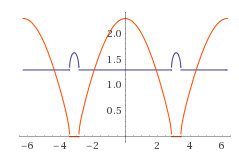
\includegraphics[width=0.4\linewidth]{img.png}
\end{figure}

\end{document}